\chapter{Density Matrices, Mixed States and Measurement}
\label{ch:density}

Measurement in quantum mechanics is intrinsically random, and Bell tests show this is unavoidable: even with $|\Psi\rangle$ known exactly, measuring $A$ gives $a_i$ with probability $|\langle i|\Psi\rangle|^2$. Uncertainty can also come from incomplete knowledge of the system, from having access to only part of it, or from a system interacting with a stochastic environment. State vectors cannot represent this second kind of randomness, so we need a new tool.

% ============================================================
\section{Ensembles}
% ============================================================

\begin{definition}[Ensemble]
An ensemble is a collection of normalized states with probabilities,
\[
    \mathcal{E} = \bigl\{(p_1,|\psi_1\rangle),\ldots,(p_n,|\psi_n\rangle)\bigr\},
    \qquad
    \sum_ip_i = 1,
    \quad
    p_i>0 .
\]
The number of members is unconstrained by $\dim V$, and the states need not be orthogonal. The expectation value of an observable is the weighted average,
\[
    \langle\hat{O}\rangle_{\mathcal{E}} = \sum_ip_i\langle\psi_i|\hat{O}|\psi_i\rangle .
\]
\end{definition}

\begin{example}[Pure and mixed ensembles]
For a spin, $\mathcal{E}_a = \{(1,|z+\rangle)\}$ is \emph{pure}. $\mathcal{E}_b = \{(\frac12,|z+\rangle),(\frac12,|z-\rangle)\}$ is \emph{mixed}, as are $\mathcal{E}_c = \{(\frac12,|z+\rangle),(\frac14,|x+\rangle),(\frac14,|y-\rangle)\}$ and the unpolarized ensemble $\mathcal{E}_d$ of $|\uvect{n}(\theta,\phi),+\rangle$ uniformly over directions.
\end{example}

An ensemble is very different from the superposition of its states: $\mathcal{E}_b$ has $\langle\hat{S}_x\rangle = 0$, while $\frac{1}{\sqrt2}(|z+\rangle + |z-\rangle) = |x+\rangle$ has $\langle\hat{S}_x\rangle = \hbar/2$. Mixed states are more general than pure states: $\mathcal{E}_b$ has $\langle\hat{S}_{\uvect{n}}\rangle = 0$ for every $\uvect{n}$, which no single state can, since every state is $|\uvect{m},+\rangle$ for some $\uvect{m}$. Different ensembles can be \emph{indistinguishable}, with all expectation values equal: $\{(\frac12,|z\pm\rangle)\}$ and $\{(\frac12,|x\pm\rangle)\}$ both give $\langle\hat{S}_{\uvect{n}}\rangle = 0$ for all $\uvect{n}$.

Mixed states also arise from entanglement. If Alice and Bob share many copies of the singlet and Alice measures $S_z$ on hers, Bob's particles are each $|+\rangle$ or $|-\rangle$ with probability $\frac12$, in an unknown order: his ensemble is $\{(\frac12,|+\rangle_B),(\frac12,|-\rangle_B)\}$.

% ============================================================
\section{Density Matrices}
% ============================================================

\begin{definition}[Density matrix]
\[
    \rho_{\mathcal{E}} = \sum_ip_i|\psi_i\rangle\langle\psi_i|,
    \qquad
    \langle\hat{Q}\rangle_{\mathcal{E}} = \operatorname{tr}(\rho_{\mathcal{E}}\hat{Q}) .
\]
\end{definition}

Ensembles are indistinguishable if and only if they have the same density matrix (if $\operatorname{tr}(\hat{Q}\Delta\rho) = 0$ for all $\hat{Q}$, take $\hat{Q} = \Delta\rho^\dagger$ to get $\Delta\rho = 0$), so the density matrix removes the redundancy in the ensemble description. Each $\rho$ arises from infinitely many ensembles (``unravellings'').

\begin{theorem}[Properties of density matrices]
$\rho$ is Hermitian, positive semi-definite ($\langle\phi|\rho|\phi\rangle = \sum_ip_i|\langle\phi|\psi_i\rangle|^2\ge0$), and has $\operatorname{tr}\rho = 1$. Conversely any such operator is a density matrix.
\end{theorem}

\begin{example}[Spin density matrices]
In the $\{|z+\rangle,|z-\rangle\}$ basis,
\[
    \rho_a = \begin{pmatrix}1&0\\0&0\end{pmatrix},
    \qquad
    \rho_b = \rho_d = \frac12\begin{pmatrix}1&0\\0&1\end{pmatrix},
    \qquad
    \rho_c = \begin{pmatrix}\frac34 & \frac{1+i}{8}\\ \frac{1-i}{8} & \frac14\end{pmatrix}.
\]
\end{example}

\begin{definition}[Purity]
\[
    \zeta(\rho) = \operatorname{tr}(\rho^2)\le1,
\]
with equality if and only if $\rho$ is pure. Indeed $\zeta = \sum_{ij}p_ip_j|\langle\psi_i|\psi_j\rangle|^2\le\sum_{ij}p_ip_j = 1$ by Schwarz, with equality only if all the states coincide up to phase. Purity is not an observable: no $\hat{Q}$ has $\operatorname{tr}(\hat{Q}\rho) = \zeta(\rho)$ for all $\rho$, since that expression is linear in $\rho$. Minimizing $\sum p_i^2$ subject to $\sum p_i = 1$ gives the \emph{maximally mixed} state $\rho = I/n$.
\end{definition}

\begin{formula}[The Bloch ball]
Every spin-$\frac12$ density matrix is
\[
    \rho = \frac12\bigl(I + \lvect{a}\cdot\bm{\sigma}\bigr),
    \qquad
    \lvect{a}\in\mathbb{R}^3,
    \qquad
    |\lvect{a}|\le1,
\]
since $\operatorname{tr}\rho = 1$, $\rho = \rho^\dagger$ and $\det\rho = \frac14(1-|\lvect{a}|^2)\ge0$. Then $\rho^2 = \frac14(1+|\lvect{a}|^2) + \frac12\lvect{a}\cdot\bm{\sigma}$, so $\rho$ is pure exactly when $|\lvect{a}| = 1$. Pure states lie on the surface of the \emph{Bloch sphere}, mixed states inside it, and the maximally mixed state $\frac12I$ at the centre.
\end{formula}

\begin{figure}[ht]
\centering
\begin{tikzpicture}[scale=1.5,>=Stealth]
  \shade[ball color=blue!10] (0,0) circle (1);
  \draw (0,0) circle (1);
  \draw[dashed] (1,0) arc (0:180:1 and 0.3);
  \draw (-1,0) arc (180:360:1 and 0.3);
  \draw[->] (0,0) -- (0,1.3) node[above]{$a_z$};
  \draw[->] (0,0) -- (1.3,0) node[right]{$a_y$};
  \draw[->] (0,0) -- (-0.7,-0.45) node[below left]{$a_x$};
  \draw[->,very thick,blue!70!black] (0,0) -- (0.6,0.8); \fill[blue!70!black] (0.6,0.8) circle (0.03) node[above right]{\small pure};
  \draw[->,very thick,red!70!black] (0,0) -- (-0.35,0.3); \fill[red!70!black] (-0.35,0.3) circle (0.03) node[above left]{\small mixed};
  \fill (0,0) circle (0.035); \node[below right] at (0,0) {\small $\frac12I$};
\end{tikzpicture}
\caption{The Bloch ball. The surface $|\lvect{a}| = 1$ holds the pure states, the interior the mixed states, and the centre the maximally mixed state. The purity is $\operatorname{tr}\rho^2 = \frac12(1+|\lvect{a}|^2)$.}
\end{figure}

The Bloch vector has a direct meaning: $\langle\bm{\sigma}\rangle = \operatorname{tr}(\rho\bm{\sigma}) = \lvect{a}$, using $\operatorname{tr}(\sigma_i\sigma_j) = 2\delta_{ij}$. So $\lvect{a}$ is the spin polarization, and $|\lvect{a}|<1$ means the spin is only partially polarized. Under a Hamiltonian $\hat{H} = -\gamma\vect{B}\cdot\hat{\lvect{S}}$, the von Neumann equation gives $\dot{\lvect{a}} = -\gamma\vect{B}\times\lvect{a}$: the whole Bloch ball rotates rigidly, preserving $|\lvect{a}|$ (purity). Decoherence instead shrinks $\lvect{a}$ toward the centre.

\begin{formula}[Ensemble from a density matrix]
A density matrix fixes all predictions, but not the ensemble: for example $\frac12I$ is produced equally by $\{(\frac12,|z\pm\rangle)\}$, by $\{(\frac12,|x\pm\rangle)\}$, and by the uniform distribution over the whole Bloch sphere. Two ensembles $\{p_i,|\psi_i\rangle\}$ and $\{q_j,|\phi_j\rangle\}$ give the same $\rho$ if and only if $\sqrt{q_j}|\phi_j\rangle = \sum_iU_{ji}\sqrt{p_i}|\psi_i\rangle$ for some unitary $U$.
\end{formula}

% ============================================================
\section{Subsystems and Reduced Density Matrices}
% ============================================================

Consider a bipartite system $\mathcal{H} = A\otimes\bar{A}$. \emph{Entangled is not the same as mixed}: the entangled $\frac{1}{\sqrt2}(|\phi_1\rangle|\chi_1\rangle + |\phi_2\rangle|\chi_2\rangle)$ is a pure state with $\operatorname{tr}\rho^2 = 1$, while $\frac12(|\psi_1\rangle\langle\psi_1| + |\psi_2\rangle\langle\psi_2|)$ built from two product states is mixed.

\begin{definition}[Reduced density matrix]
For observables acting only on $A$, $\hat{Q} = \hat{Q}_A\otimes I_{\bar{A}}$, all expectation values follow from the \emph{partial trace}
\[
    \rho_A = \operatorname{tr}_{\bar{A}}\rho = \sum_k\,{}_{\bar{A}}\langle k|\rho|k\rangle_{\bar{A}},
    \qquad
    \operatorname{tr}_A(\rho_A\hat{Q}_A) = \operatorname{tr}(\rho\hat{Q}).
\]
$\rho_A$ is itself a density matrix.
\end{definition}

For a product state $|\phi\rangle_A|\chi\rangle_{\bar{A}}$, $\rho_A = |\phi\rangle\langle\phi|$ is pure. For the entangled $\frac{1}{\sqrt2}(|01\rangle - |10\rangle)$, $\rho_A = \frac12(|0\rangle\langle0| + |1\rangle\langle1|)$ is mixed: an entangled state looks mixed to a local observer, because information about the whole is missing locally. Conversely any $\rho_A = \sum_\alpha\lambda_\alpha|\psi_\alpha\rangle\langle\psi_\alpha|$ is the reduced density matrix of the pure state $|\Psi\rangle = \sum_\alpha\sqrt{\lambda_\alpha}|\psi_\alpha\rangle_A|\phi_\alpha\rangle_{\bar{A}}$ (with orthonormal $|\phi_\alpha\rangle$), a \emph{purification} of $\rho_A$.

\begin{example}[Partial trace step by step]
For $|\Psi\rangle = \frac{1}{\sqrt2}(|01\rangle - |10\rangle)$,
\[
    \rho = \tfrac12\bigl(|01\rangle\langle01| - |01\rangle\langle10| - |10\rangle\langle01| + |10\rangle\langle10|\bigr).
\]
The partial trace over $\bar{A}$ uses $\operatorname{tr}_{\bar{A}}\bigl(|ab\rangle\langle cd|\bigr) = |a\rangle\langle c|\,\langle d|b\rangle$. The cross terms have $b\neq d$ and vanish, leaving
\[
    \rho_A = \tfrac12\bigl(|0\rangle\langle0| + |1\rangle\langle1|\bigr) = \tfrac12I,
\]
maximally mixed, with purity $\frac12$. Every local measurement on $A$ gives completely random results, even though the whole state is pure: all the information is in the correlations.
\end{example}

\begin{example}[Partially entangled state]
For $|\Psi\rangle = \cos\theta|00\rangle + \sin\theta|11\rangle$, $\rho_A = \cos^2\theta|0\rangle\langle0| + \sin^2\theta|1\rangle\langle1|$ with purity $\cos^4\theta + \sin^4\theta$. This is already a Schmidt decomposition with coefficients $\cos\theta$, $\sin\theta$. A natural measure of entanglement is the entropy of $\rho_A$, $S = -\operatorname{tr}\rho_A\ln\rho_A = -\cos^2\theta\ln\cos^2\theta - \sin^2\theta\ln\sin^2\theta$, which vanishes for product states ($\theta = 0$) and is maximal, $\ln2$, for a Bell state ($\theta = \pi/4$).
\end{example}

\begin{theorem}[Schmidt decomposition]
Any pure state of $\mathcal{H}_A\otimes\mathcal{H}_B$ (with $d_A\le d_B$) can be written
\[
    |\Psi_{AB}\rangle = \sum_{i=1}^{\chi}\lambda_i|i\rangle_A\otimes|i'\rangle_B,
    \qquad
    \lambda_i\ge0,
\]
with $\{|i\rangle_A\}$ orthonormal and $\{|i'\rangle_B\}$ an orthonormal set. The reduced density matrices are then diagonal with the same spectrum, $\rho_A = \sum_ip_i|i\rangle\langle i|$ and $\rho_B = \sum_ip_i|i'\rangle\langle i'|$ with $p_i = \lambda_i^2$.
\end{theorem}
\begin{proof}[Sketch]
Diagonalize $\rho_A = \sum_ip_i|i\rangle\langle i|$ and write $|\Psi\rangle = \sum_i|i\rangle_A|\tilde{i}\rangle_B$. Computing $\rho_A$ from this form shows ${}_B\langle\tilde{j}|\tilde{i}\rangle_B = p_i\delta_{ij}$, so $|i'\rangle = |\tilde{i}\rangle/\sqrt{p_i}$ are orthonormal.
\end{proof}

The \emph{Schmidt rank} $\chi$, with $1\le\chi\le\min(d_A,d_B)$, measures how entangled the state is: $\chi = 1$ exactly for product states.

\begin{example}[Finding a Schmidt decomposition]
Take $|\Psi\rangle = \frac{1}{\sqrt3}\bigl(|00\rangle + |01\rangle + |10\rangle\bigr)$, with coefficient matrix $\psi = \frac{1}{\sqrt3}\begin{pmatrix}1&1\\1&0\end{pmatrix}$. Then $\rho_A = \psi\psi^\dagger = \frac13\begin{pmatrix}2&1\\1&1\end{pmatrix}$, with eigenvalues $p_\pm = \frac12\pm\frac{\sqrt5}{6}\approx0.873,\ 0.127$. The Schmidt coefficients are $\lambda_\pm = \sqrt{p_\pm}$, the Schmidt rank is 2 (entangled), and the eigenvectors of $\rho_A$ and of $\rho_B = \psi^T\psi^*$ give the Schmidt bases. This is the singular value decomposition of the matrix $\psi$.
\end{example}

\begin{theorem}[No-communication theorem]
Nothing Bob does to his half of an entangled pair changes Alice's reduced density matrix, so entanglement cannot be used to send signals.
\end{theorem}
\begin{proof}
If Bob applies a unitary $U_B$, then $\rho_A' = \operatorname{tr}_B\bigl[(I\otimes U_B)\rho(I\otimes U_B^\dagger)\bigr] = \operatorname{tr}_B\rho = \rho_A$ by cyclicity of the partial trace over $B$. If Bob measures with projectors $P_k$ and does not tell Alice the result, $\rho_A' = \sum_k\operatorname{tr}_B[(I\otimes P_k)\rho(I\otimes P_k)] = \operatorname{tr}_B\bigl[\rho\sum_kP_k\bigr] = \rho_A$.
\end{proof}

This is why teleportation needs the two classical bits: until Bob receives them, his qubit is in the maximally mixed state $\frac12I$, carrying no information about $|\psi\rangle$.

% ============================================================
\section{Thermal States}
% ============================================================

A system in equilibrium with a heat bath at temperature $T$ is in the mixed state
\[
    \rho = \frac{e^{-\beta\hat{H}}}{Z},
    \qquad
    Z = \operatorname{tr}e^{-\beta\hat{H}} = \sum_ne^{-\beta E_n},
    \qquad
    \beta = \frac{1}{k_BT},
\]
i.e.\ the ensemble $\{(e^{-\beta E_n}/Z,|n\rangle)\}$ of energy eigenstates with Boltzmann weights. It commutes with $\hat{H}$, so it is stationary, and it maximizes the von Neumann entropy $S = -k_B\operatorname{tr}\rho\ln\rho$ at fixed $\langle\hat{H}\rangle$. As $T\to0$ it becomes the pure ground state; as $T\to\infty$ it becomes maximally mixed.

\begin{example}[Thermal spin]
For $\hat{H} = -\mu B\sigma_z$, $\rho = \frac{1}{2\cosh\beta\mu B}\operatorname{diag}(e^{\beta\mu B},e^{-\beta\mu B}) = \frac12(I + \tanh(\beta\mu B)\sigma_z)$. The Bloch vector points along $\vect{B}$ with length $\tanh(\mu B/k_BT)$, and the magnetization $\langle\mu\sigma_z\rangle = \mu\tanh(\mu B/k_BT)\approx\mu^2B/k_BT$ at high temperature: Curie's law.
\end{example}

\begin{figure}[ht]
\centering
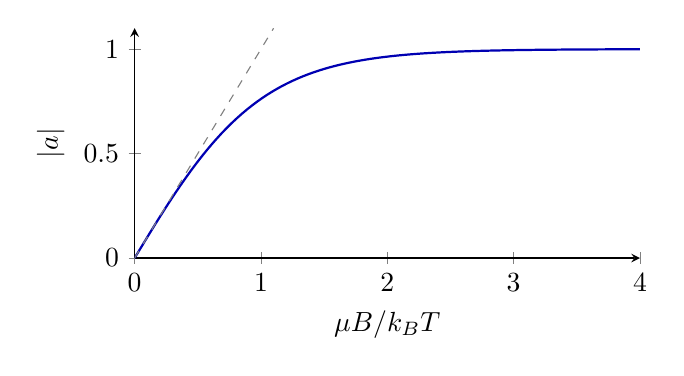
\begin{tikzpicture}
\begin{axis}[width=8cm,height=4.5cm,xlabel={$\mu B/k_BT$},ylabel={$|\lvect{a}|$},axis lines=left,xmin=0,xmax=4,ymin=0,ymax=1.1,domain=0:4,samples=100]
\addplot[thick,blue!70!black]{tanh(x)};
\addplot[dashed,gray,domain=0:1.1]{x};
\end{axis}
\end{tikzpicture}
\caption{Polarization of a thermal spin: linear (Curie) at high temperature, saturating at a pure state as $T\to0$.}
\end{figure}

% ============================================================
\section{Dynamics and Measurement}
% ============================================================

Under unitary evolution each ensemble member evolves, so
\[
    \rho(t) = U(t,t_0)\rho(t_0)U^\dagger(t,t_0).
\]

\begin{formula}[von Neumann equation]
\[
    i\hbar\frac{d}{dt}\rho(t) = [\hat{H}(t),\rho(t)].
\]
Unitary evolution preserves $\operatorname{tr}\rho$, positivity, and the purity $\operatorname{tr}\rho^2$.
\end{formula}

\begin{proof}[Derivation of the von Neumann equation]
Differentiate $\rho(t) = U\rho(t_0)U^\dagger$ using $i\hbar\dot{U} = \hat{H}U$ and $-i\hbar\dot{U}^\dagger = U^\dagger\hat{H}$:
\[
    i\hbar\dot\rho = \hat{H}U\rho(t_0)U^\dagger - U\rho(t_0)U^\dagger\hat{H} = [\hat{H},\rho].
\]
Note the sign: this is the opposite of the Heisenberg equation for an operator, because $\rho$ is built from states, which evolve in the Schr\"odinger picture. Purity is conserved because $\operatorname{tr}(U\rho U^\dagger U\rho U^\dagger) = \operatorname{tr}(\rho^2)$ by cyclicity.
\end{proof}

\begin{formula}[Measuring a mixed spin]
For $\rho = \frac12(I + \lvect{a}\cdot\bm{\sigma})$ and a measurement of $\uvect{n}\cdot\bm{\sigma}$, with projectors $P_\pm = \frac12(I\pm\uvect{n}\cdot\bm{\sigma})$: $p(\pm) = \operatorname{tr}(\rho P_\pm) = \frac12(1\pm\uvect{n}\cdot\lvect{a})$. After recording $+$, the state is the pure $|\uvect{n},+\rangle$; after measuring and forgetting, $\tilde\rho = \frac12\bigl(I + (\uvect{n}\cdot\lvect{a})\,\uvect{n}\cdot\bm{\sigma}\bigr)$: the Bloch vector is projected onto the measurement axis.
\end{formula}

\paragraph{Measurement.} Write $\hat{O} = \sum_\alpha\lambda_\alpha P_\alpha$. The outcome $\lambda_\alpha$ occurs with probability $p(\alpha) = \operatorname{tr}(\rho P_\alpha)$.
\begin{itemize}
    \item \emph{Measure and record the outcome}: $\rho\to\rho_\alpha = P_\alpha\rho P_\alpha/p(\alpha)$.
    \item \emph{Measure and forget the outcome}: $\rho\to\tilde\rho = \sum_\alpha P_\alpha\rho P_\alpha$. For example, measuring $S_z$ on $\frac{1}{\sqrt2}(|z+\rangle + |z-\rangle)$ and forgetting the result leaves the maximally mixed $\frac12I$.
\end{itemize}

In real systems, stray single electrons and photons make untracked ``measurements'' all the time, which is equivalent to forgetting. So states \emph{decohere} into mixed states unless extraordinary efforts are made, which is why quantum computers are so hard to build. More generally, interaction with an environment $\bar{A}$ makes the evolution of a subsystem non-unitary: purify $\rho_A$ to $|\Psi\rangle\langle\Psi|$ on $A\otimes\bar{A}$, evolve unitarily, and trace out the environment again. This ``quantum channel'' is modelled by the Lindblad master equation.

\begin{example}[A model of decoherence]
A qubit $\alpha|0\rangle + \beta|1\rangle$ interacts with an environment qubit, initially $|e\rangle$, such that $|0\rangle|e\rangle\to|0\rangle|e_0\rangle$ and $|1\rangle|e\rangle\to|1\rangle|e_1\rangle$, with overlap $\langle e_0|e_1\rangle = \gamma$. Tracing out the environment,
\[
    \rho_A = \begin{pmatrix}|\alpha|^2 & \alpha\beta^*\gamma^*\\ \alpha^*\beta\gamma & |\beta|^2\end{pmatrix}.
\]
The populations are untouched but the coherences are multiplied by $\gamma$. If the environment records which state the qubit is in ($\gamma\to0$), the qubit becomes the mixture $\operatorname{diag}(|\alpha|^2,|\beta|^2)$: the result of a measurement whose outcome nobody read. With $N$ environment qubits each contributing an overlap $\gamma_1<1$, $\gamma = \gamma_1^N$ decays exponentially in $N$, which is why macroscopic superpositions decohere almost instantly.
\end{example}

\paragraph{What is a measurement?} Isolated systems evolve unitarily, but measurement is probabilistic. Does quantum mechanics describe an objective reality, or an observer's perception of it? There is no consensus. One plausible account uses \emph{pointer states}. A system $S$ with $\hat{O}_S|s_i\rangle = s_i|s_i\rangle$ in a state $\sum_ic_i|s_i\rangle$ is coupled to an apparatus $A$ in a ready state $|a_0\rangle$ by $\hat{H} = \lambda\hat{O}_S\hat{P}_A$, where $\hat{P}_A$ translates the pointer. After a time $\tau$ this \emph{premeasurement} gives
\[
    \sum_ic_i|s_i\rangle\otimes|a_0 + \lambda\tau s_i/\hbar\rangle,
\]
correlating each system eigenstate with a pointer position. An environment with many degrees of freedom then becomes entangled too, with nearly orthogonal states $\langle E_i|E_j\rangle\approx\delta_{ij}$, so tracing it out leaves
\[
    \rho_{SA}\approx\sum_i|c_i|^2|s_i\rangle|a_i\rangle\langle s_i|\langle a_i|,
\]
the ensemble $\{(|c_i|^2,|s_i\rangle|a_i\rangle)\}$ of definite outcomes. In the \emph{many-worlds} interpretation there is never any non-unitary evolution: at each measurement the state branches into all outcomes, each realized in its own non-interacting ``world'', and the apparent randomness is just which branch we find ourselves in.

\begin{fact}[Key results of this chapter]
\leavevmode
\begin{itemize}
\item Mixed states are density matrices $\rho = \sum p_i|\psi_i\rangle\langle\psi_i|$: Hermitian, positive, unit trace; $\langle Q\rangle = \operatorname{tr}(\rho Q)$.
\item Purity $\operatorname{tr}\rho^2\le1$; qubits fill the Bloch ball.
\item Subsystems of entangled states are mixed: $\rho_A = \operatorname{tr}_B\rho$; Schmidt decomposition.
\item $i\hbar\dot\rho = [\hat{H},\rho]$; measurement projects; decoherence kills off-diagonal elements.
\end{itemize}
\end{fact}
